
\documentclass[smallcondensed]{svjour3}    % onecolumn (standard format)

%\documentclass[smallextended]{svjour3}     % onecolumn (second format)

%\documentclass[twocolumn]{svjour3}         % twocolumn

%
\smartqed  % flush right qed marks, e.g. at end of proof


%
% insert here the call for the packages your document requires

%
\usepackage{graphicx}
%
\usepackage{mathptmx}      
\usepackage{amsmath}

%\usepackage{latexsym}
% etc.

%%%%%%%%%%%     IMPORTANT
%
% please place your own definitions here and don't use \def but
% \newcommand{}{}

\newcommand{\NumPlanetsConfirmed}{195}
\newcommand{\NumPlanetsMinMassOK}{148}
\newcommand{\NumPlanetsMinMassNotOK}{47}
\newcommand{\NumKeplerPlanetsPleTen}{1652}
\newcommand{\NumKeplerPlanetsPleOne}{111}
\newcommand{\NumSmallKeplerPlanetsPleOne}{85}
\newcommand{\NumLargePlanetsPleTen}{23}
\newcommand{\binsize}{10-min}
\newcommand{\mediumprecision}{600 ppm}
\newcommand{\newprecision}{80 ppm}
\newcommand{\boxcarwidth}{0.5 days}
\newcommand{\numbins}{50}

\newcommand{\tess}{\emph{TESS}}
\newcommand{\kepler}{\emph{Kepler}}
\newcommand{\corot}{\emph{CoRoT}}
\newcommand{\ktwo}{\emph{K2}}

%%%%%%%%%% 56


\begin{document}


\title{Tidal Decay and Disruption of Short-Period Gaseous Exoplanets}
%\subtitle{Do you have a subtitle? \\ If so, write it here}


%\titlerunning{Short form of title} % if too long for running head


\author{Brian Jackson         \and
        Emily Jensen %etc.
}


%\authorrunning{Short form of author list} % if too long for running head


\institute{Brian Jackson \at
		Boise State University, Dept.\ of Physics\\              
		1910 University Drive, Boise ID 83725 USA \\
		Tel.: 208-426-3723\\
              \email{bjackson@boisestate.edu} }        
\maketitle


\begin{abstract}
Many gaseous exoplanets in short-period orbits are on the verge or are
actually in the process of tidal disruption. Moreover, orbital
stability analysis shows tides can drive most known hot Jupiters to
spiral inexorably into their host stars. Thus, the coupled processes
of orbital decay and tidal disruption likely shape the observed
distribution of close-in exoplanets and may even be responsible for
producing the shortest-period rocky planets. However, the exact
outcome for a disrupting planet depends on its internal response to
mass loss and variable stellar insolation, and the accompanying
orbital evolution can act to enhance or inhibit the disruption
process, depending on the geometry of the atmospheric outflow. In some
cases, strong stellar insolation can produce a deep radiative zone in
a planet's atmosphere, which can also influence the disruption and
therefore the orbital evolution. Understanding these coupled processes
and making accurate predictions requires a model that includes both
the internal and the orbital evolution of the planet. In this
presentation, we will discuss our preliminary work on tidal decay and
disruption of close-in gas giants using the fully-featured and robust
Modules for Experiments in Stellar Astrophysics (MESA) suite, the
capabilities of which were recently upgraded to model gaseous planets
with inert, rocky cores.
\keywords{First keyword \and Second keyword \and More}
% \PACS{PACS code1 \and PACS code2 \and more}

\end{abstract}


\section{Introduction}
\label{sec:introduction}

\section{Introduction}

\begin{figure}
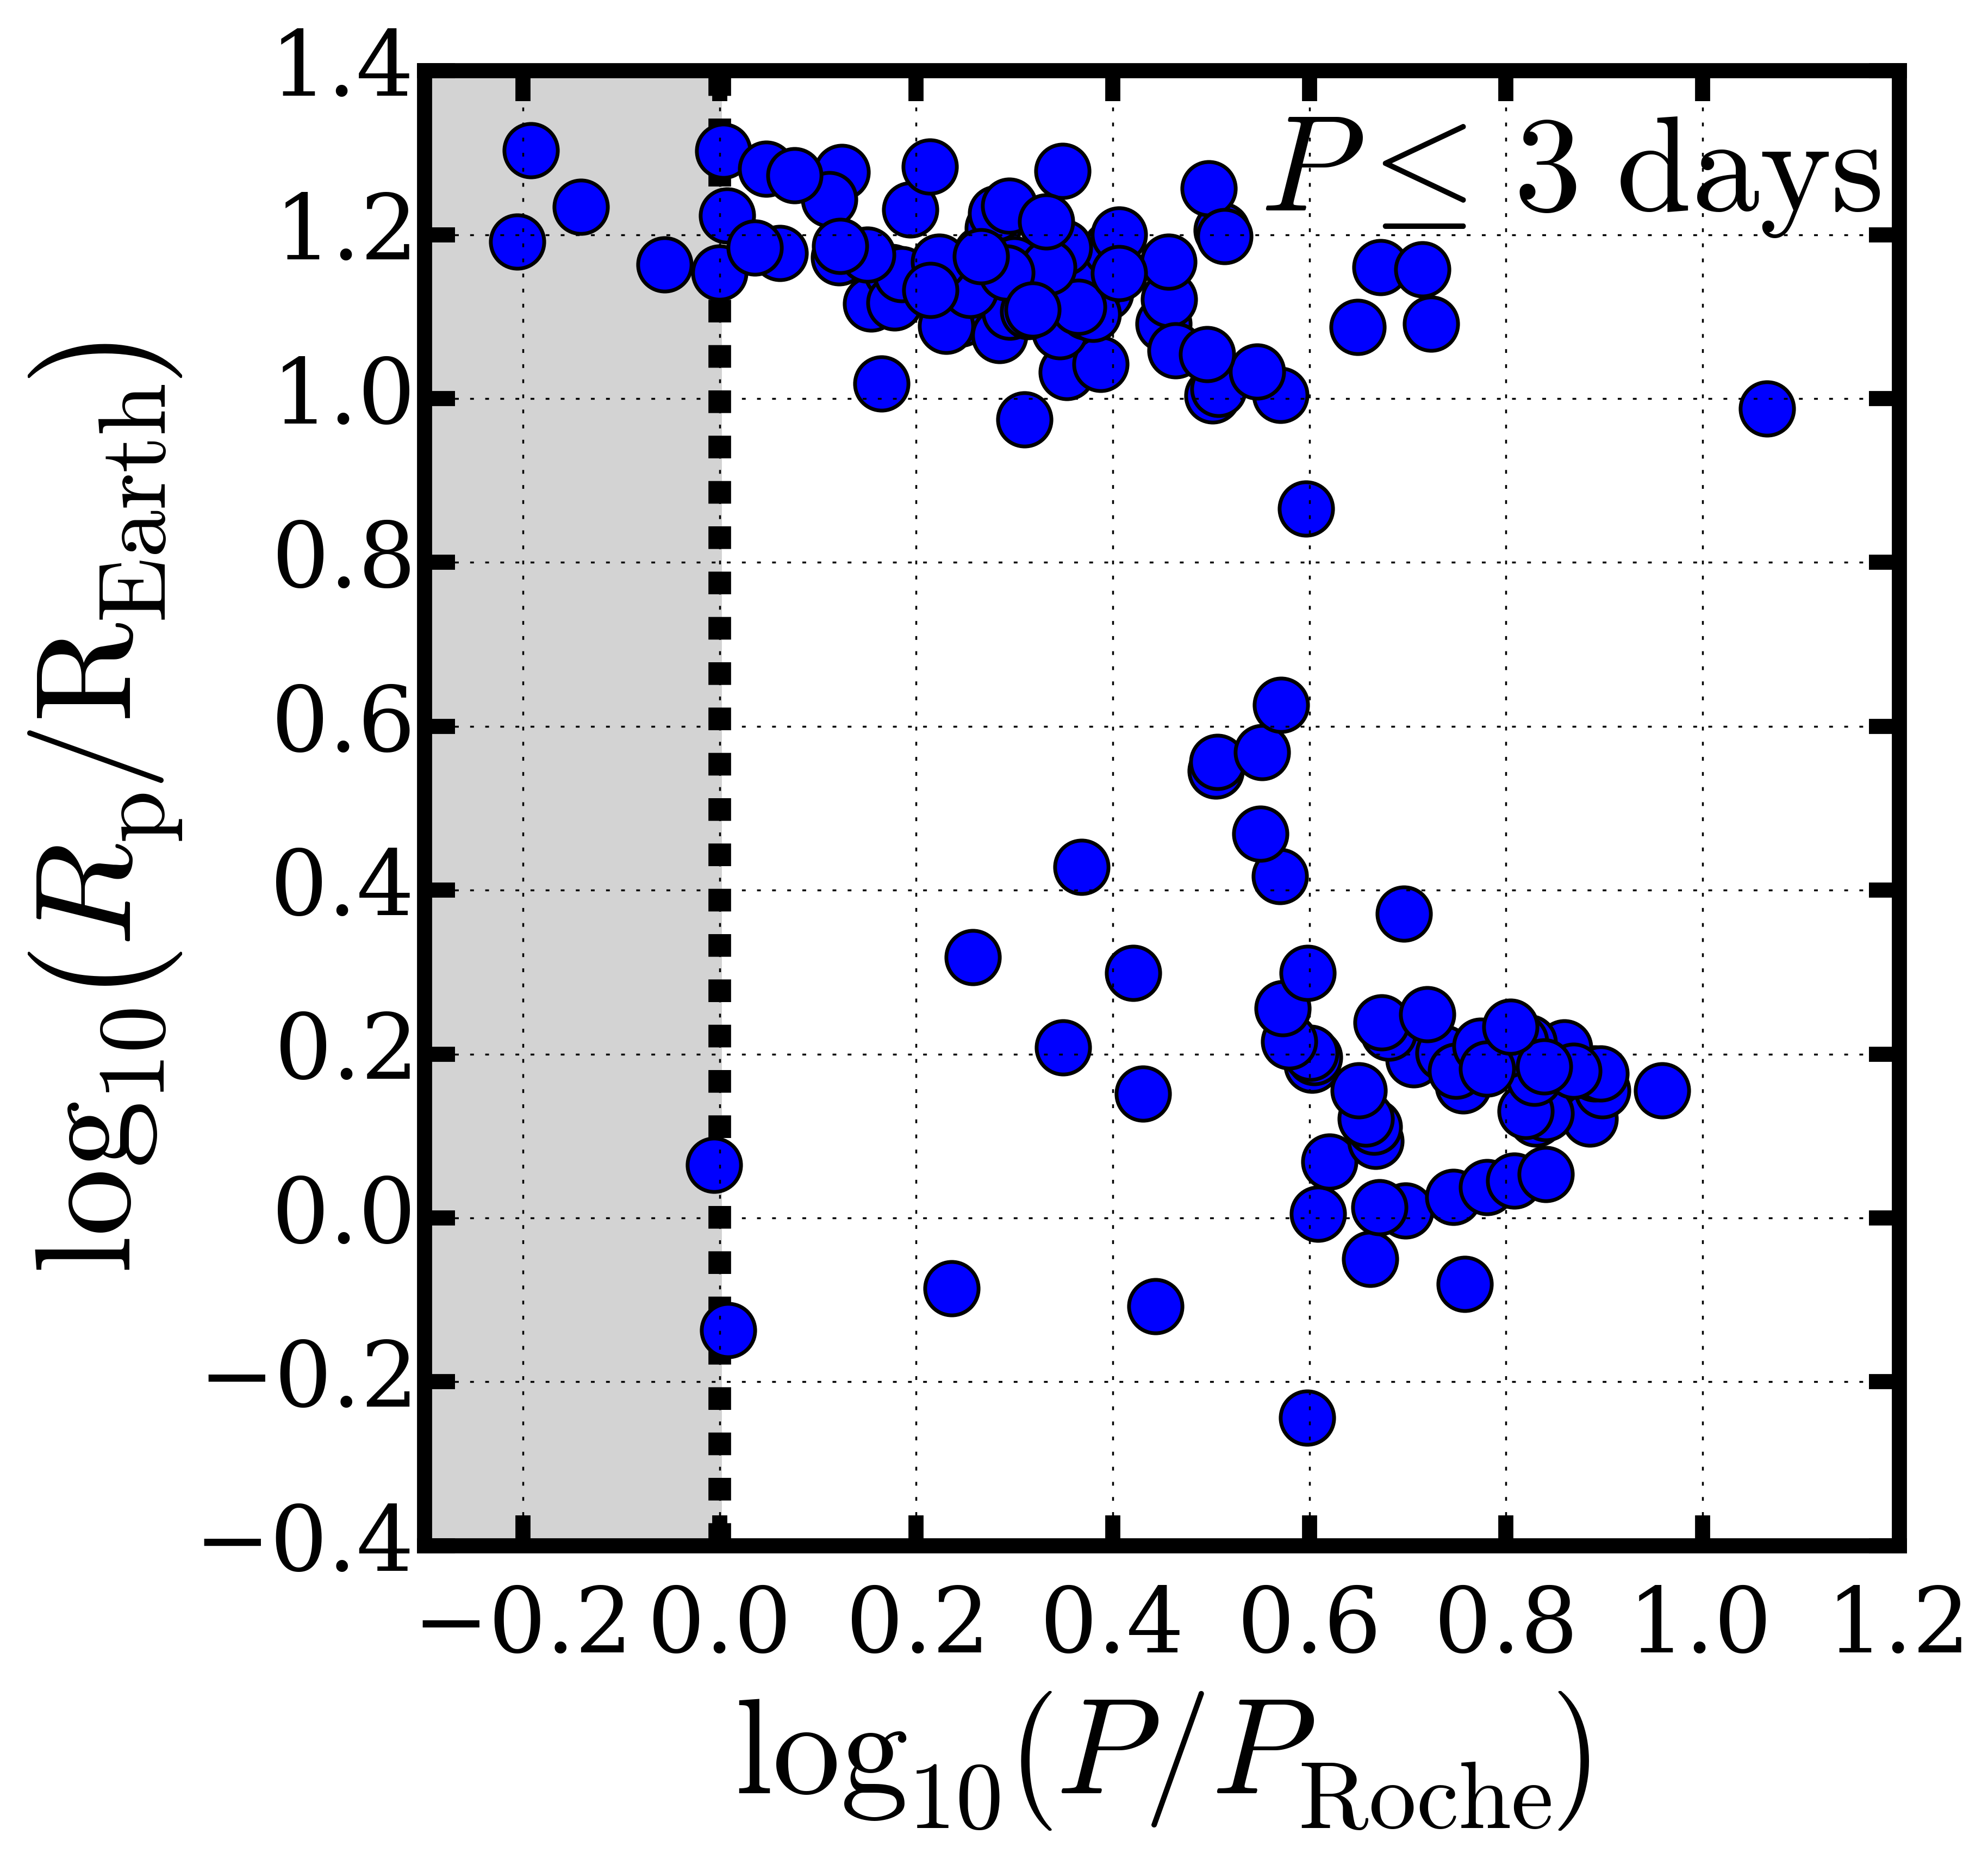
\includegraphics[width=\textwidth]{P-PRoche.png}
\caption{Planetary radius $R_{\rm p}$ in Earth radii ($R_{\rm Earth}$) vs. the ratio of orbital period $P$ to its Roche period $P_{\rm Roche}$ for $P \leq$ 3 days. Data collected from exoplanets.org on 2015 Dec 7.}
\label{fig:P-PRoche}
\end{figure}

The following lines of evidence point to or are at least consistent with tidal decay and subsequent atmospheric disruption of short-period gaseous exoplanets:

\begin{enumerate}
\item The majority of hot Jupiters are formally unstable against tidal decay.
%Re-work Rick's analysis for non-zero obliquity?
%Updated plot of Levrard's analysis

\item Among the many \kepler\ targets for which rotation periods have been estimated, short-period planets are less commonly observed transiting the most rapidly rotating stars.
%How much angular momentum delivered? How much change stellar rotation rate?

\item Poppenhaeger \& Wolk (20XX) estimated x-ray activity (which scales with stellar rotation frequency) for several widely separated binary stars in which one of the stars hosted a short-period planet and the other did not. Those stars with relatively deep convective zones exhibited enhanced x-ray activity, and hence more rapid rotation, than expected based on the x-ray activity of the partner stars without planets. 
%F-M's analysis

\item There is a dearth of super-Earth/sub-Neptune gas-rich planets in the shortest orbital periods compared to longer orbital periods. This observation has been attributed to photoevaporative loss of the atmospheres, though.

\end{enumerate}

The following lines of evidence argue against tidal decay and subsequent atmospheric disruption of short-period gaseous exoplanets:

\begin{enumerate}

\item No short-period planets are currently observed undergoing disruption.
%Constrain the rate of decay/disruption from this fact?

\item Where are the remnants of decay/disruption? The population of small ultra-short period planets are too close to be the remnants.

\end{enumerate}

As a first approximation to the mass-period relationship expected for the remnants, we use the $M_{\rm p}-R_{\rm p}$ relationship for sub-Neptunes provided in \cite{}, produced by fitting a combination of power laws to their more detailed atmospheric models:
\begin{equation}
R_{\rm p} \approx 2.06\ {\rm R_{Earth}}\ \left( \dfrac{M_{\rm p}}{\rm M_{Earth}} \right)^{-0.21} \left( \dfrac{f_{\rm env}}{0.05\%} \right)^{0.59} \left( \dfrac{F_{\rm p}}{\rm F_{Earth}} \right)^{0.044} \left( \dfrac{\rm age}{\rm 5\ Gyrs} \right)^{-0.18} + 1\ {\rm R_{Earth}}\  \left( \dfrac{M_{\rm core}}{\rm M_{Earth}} \right)^{0.25},
\label{eqn:LopezFortney2013_subNeptune_relation}
\end{equation}
where $f_{\rm env}$ is the fraction of the planet's mass in the gaseous envelope, $F_{\rm p}$ the stellar insolation received by the planet, and $R_{\rm core}$ is the radius of the planet's solid, rocky core. Equation \ref{eqn:LopezFortney2013_subNeptune_relation} involves a number of approximations, including neglecting the contribution to $R_{\rm p}$ of a radiative outer atmosphere, which \cite{} indicate is usually small ($0.1\ {\rm R_{Earth}}$).  The last term represents the radius of the solid core, which is insensitive to the exact proportion of iron and rock.

%\begin{acknowledgements}
%If you'd like to thank anyone, place your comments here
%and remove the percent signs.

%\end{acknowledgements}

\bibliography{Jackson_tidal-decay-disrupt}

\end{document}